Here the problem is the same as in the previous step, the only difference is that not only the conversion rates of the customers are unknown, but also the alpha ratios and the number of products sold for each price.
Since the learners are not able to distinguish the different types of customers, initially the alphas values (probability to start the interaction from a specific product) are uniformly distributed ($[0.2, 0.2, 0.2, 0.2, 0.2]$) and the number of products bought for each price is set all to 1.\\
The same algorithm as before has been developed, with the additional capability of estimating the two parameters, that are now uncertain.

\subsection{UCB-1}
The algorithm repeats the same operation as in the previous chapter from step 1 to step 5. Then, it estimates the two parameters:

\begin{itemize}
    \item estimate alpha ratios:\begin{equation}
        \label{eqn:alpha}
        \alpha = \alpha + starts
    \end{equation}where starts is a vector that collects the number of times a customer start from a specific product to visit the web page
    \item estimate number of products sold (version 1):\\
    with this first approach, we evaluate these parameters with the empirical mean as can be seen in Equation ~\ref{eqn:num_prod} \begin{equation}
        \label{eqn:mean_items}
        mean\_items[p,a] = \frac{mean\_items[p,a] * seen[p,a] + bought[p]}{estimated\_items[p,a]}
    \end{equation}\begin{equation}
        \label{eqn:num_prod}
        num\_products[p,a] = \frac{1}{mean\_items[p,a]}
    \end{equation}where\begin{itemize}
        \item mean\_items[p,a] in the mean of the number of products {\bf p} with price {\bf a} has been bought till now
        \item seen[p,a] is the number of times products {\bf p} with price {\bf a} has been bought until the day before
        \item bought[p] is the total amount of products {\bf p} bought today
        \item estimated\_items[p,a] is the number of times products {\bf p} with price {\bf a} has been bought until now (so it is seen[p,a] plus the number of times product p has been bought today)
        \item num\_products[p,a] is the inverse of the value calculated before because represents the parameters of the Geometric distribution, we have used to estimate the number of items bought from the customers, once they have decided to buy that product visualized with that price
    \end{itemize}
    \item estimate number of products sold (version 2):\\
    the calculus of the mean number of products (mean\_items[p,a]) is the same as the other version, so calculated as in Equation ~\ref{eqn:mean_items}. The difference is in the calculus of the parameter of the Geometric distribution, which is done by using a MAB. In this version of the learner, there are two additional parameters for the mean and the upper bound of these parameters we are trying to estimate. The upper bounds are updated after the Equation ~\ref{eqn:mean_items} and the means when the algorithm wants to evaluate which is the best super arm to pull. The results of this version are not shown below, because are much worse.
\end{itemize}
\subsubsection{Results}
As expected, having less knowledge leads to a solution a little bit worst compared to the previous step. In other words, the UCB Learner needs more days to converge to the optimal solution. As said before, someday it will change the super arm to pull in order to explore more.
\begin{figure}[ht]
    \begin{center}
    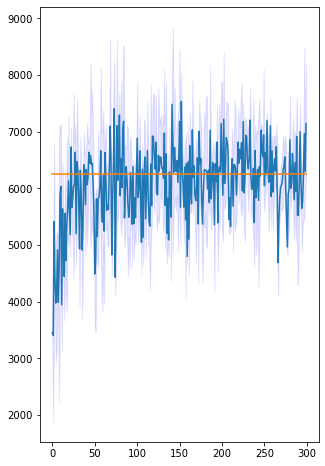
\includegraphics[width=0.6\textwidth]{img/UCB4.png}
    \caption{UCB Reward}
    \label{fig:reward41}
    \end{center}
\end{figure}
\begin{multicols}{2}
    \begin{figure}[H]
        \begin{center}
        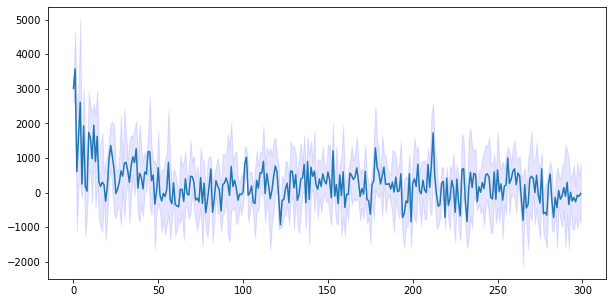
\includegraphics[width=0.5\textwidth]{img/UCB4_regret.png}
        \caption{UCB Regret}
        \label{fig:regret41}
        \end{center}
    \end{figure}
    \columnbreak
    \begin{figure}[H]
        \begin{center}
        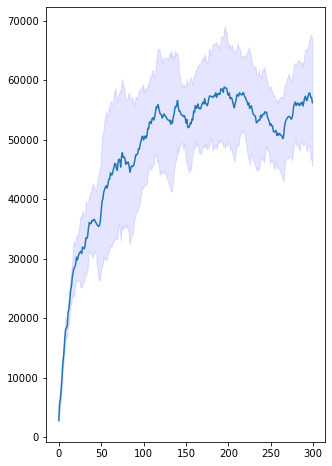
\includegraphics[width=0.5\textwidth]{img/UCB4_cum_reg.png}
        \caption{UCB Cumulative regret}
        \label{fig:cum_reg41}
        \end{center}
    \end{figure}
\end{multicols}

\subsection{TS}
Thomson Sampling estimates the alpha ratios exactly as the UCB with the Equation ~\ref{eqn:alpha}.\\About the estimation of the number of products sold, the method adopted is the same as the second version for the UCB-1. For obvious reasons, the additional parameters are the $\alpha$ and $\beta$ parameters of the Beta distribution used for the additional MAB. The update of these two is done as follows:\\\\
$\alpha[p, a]$ = $\alpha[p, a]$ + tot\_bought$[p]$\\
where tot\_bought [p] is the total amount of products {\bf p} bought from the first day until now\\\\
$\beta[p, a]$ = $\beta [p, a]$ + seen$[p]$\\
where seen [p] is the number of times the product {\bf p} has been bought until now\\\\
Also here the two parameters calculated above, are updated inside the customer attributes when the learner has to select which super arm to pull.

\subsubsection{Results}
The same as UCB can be observed here, more uncertainty leads to much time to converge. Even this time the results highlight the fact that TS performs better than UCB because takes less time to converge, and generates less cumulative regret.
\begin{figure}[ht]
    \begin{center}
    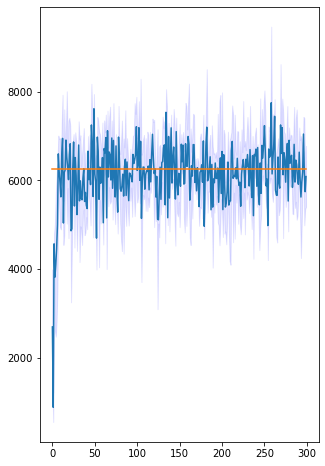
\includegraphics[width=0.6\textwidth]{img/TS4.png}
    \caption{TS Reward}
    \label{fig:reward42}
    \end{center}
\end{figure}
\begin{multicols}{2}
    \begin{figure}[H]
        \begin{center}
        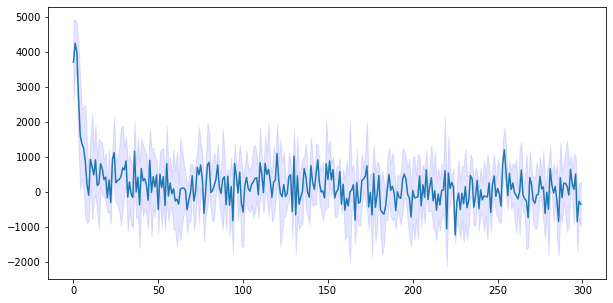
\includegraphics[width=0.5\textwidth]{img/TS4_regret.png}
        \caption{TS Regret}
        \label{fig:regret42}
        \end{center}
    \end{figure}
    \columnbreak
    \begin{figure}[H]
        \begin{center}
        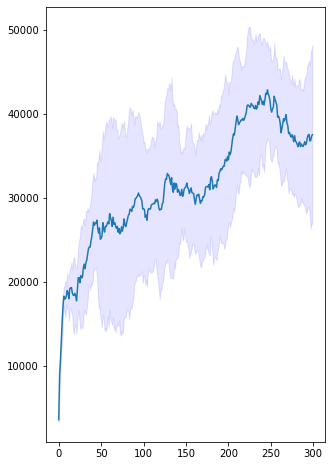
\includegraphics[width=0.5\textwidth]{img/TS4_cum_reg.png}
        \caption{TS Cumulative regret}
        \label{fig:cum_reg42}
        \end{center}
    \end{figure}
\end{multicols}
